\documentclass{beamer}
%\usetheme{Rochester}
\usepackage{graphicx}
\setbeamerfont{footnote}{size=\tiny}
\beamertemplatenavigationsymbolsempty
\title[Integer Factorisation with Elliptic Curves over Finite Fields]{Integer Factorisation with Elliptic Curves over Finite Fields}
\author{Will Bolton}
\date{February 16, 2016}

\begin{document}
\titlepage % SLIDE 0
\begin{frame} % SLIDE 1
\frametitle{Fields and finite fields}
\begin{definition}
	A field is a commutative, unital ring in which every non-zero element is invertible
\end{definition}
\vfill
	The group $\mathbb{Z}_n$ is a field if and only if $n$ is prime.
\end{frame}

\begin{frame} % SLIDE 2
\frametitle{The Euclidean Algorithm}
\begin{definition}
	The euclidean algorithm takes two numbers and returns their \emph{greatest common divisor (gcd)} by repeated division with remainder.
\end{definition}
\begin{align*}
	\gcd(21,15):21 &= 1\times15 + 6\\
	15 &= 2\times6 + 3\\
	6 &= 2\times3 + 0\\
\end{align*}
So $\gcd(21,15)=3$
\end{frame}

\begin{frame} % SLIDE 3
\frametitle{The Euclidean Algorithm}
Using the steps of the algorithm, it is possible to calculate
\begin{align*}
	\gcd(21,15) = 3 &= 1\times15 - 2\times6\\
	&= 15 - 2\times(21 - 1\times15)\\
	&= 15 - 2\times21 + 2\times15\\
	&=3\times15 - 2\times21
\end{align*}
So $3 = 3\times15 - 2\times21$
\end{frame}

\begin{frame} % SLIDE 4
\frametitle{Elliptic curves and the projective plane}
\begin{definition}
	The projective plane is an extension of regular 2-dimensional euclidean space by adding ``points at infinity'' such that every pair of lines intersects exactly once.
\end{definition}
\begin{definition}
	An elliptic curve is a non-singular cubic projective curve. For our purposes, they can all be written as $y^2 = f(x)$, where $f(x)$ is a cubic polynomial in $x$ with no repeated roots.
\end{definition}
\end{frame}

\begin{frame} % SLIDE 5
\frametitle{The elliptic curve addition law}
The points on an elliptic curve can be turned into a group via the ``chord-tangent law''
\begin{figure}[htpb]
	\centering
	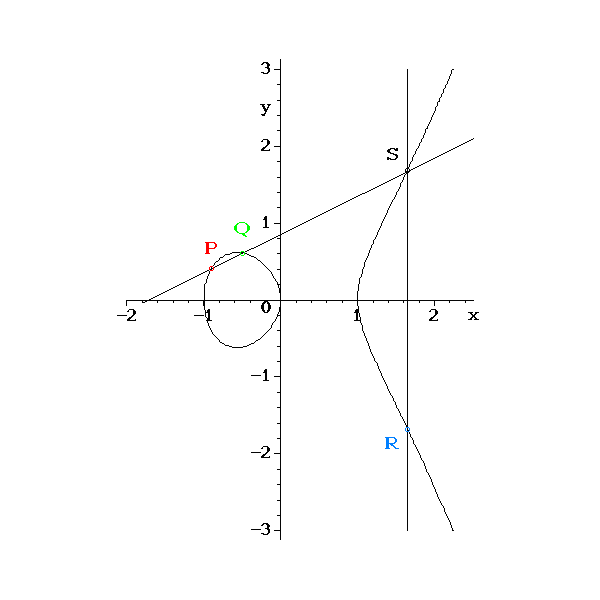
\includegraphics[scale=0.25]{addition.png}
	\caption{The addition law on an elliptic curve\footnote{Diagram taken from http://crypto.stackexchange.com/questions/11518/what-is-so-special-about-elliptic-curves}}
\end{figure}
\end{frame}

\begin{frame} % SLIDE 6
\frametitle{The elliptic curve addition law}
For elliptic curves over a finite field $\mathbb{F}_p$, when adding points $(x_1,y_1) + (x_2,y_2) = (x',y')$,
$$x'=\lambda^2 - a - x_1 - x_2,\quad y' = \lambda x_1 -\lambda x' - y_1 $$
where $\lambda = \frac{y_2-y_1}{x_2-x_1}$ if $x_1\neq x_2$ or $\lambda=\frac{3x_1^2 + 2ax_1 + b}{2y_1}$ otherwise.
\end{frame}

\begin{frame} % SLIDE 7
\frametitle{Lenstra's algorithm}
\begin{definition}
	Lenstra's algorithm goes roughly as follows to factor an integer $N$:
	\begin{itemize}
		\item Choose random integers $b$, $x$ and $y \mod N$
		\item Let $P = (x,y)$ and $c:=y^2-x^3-bx$ such that $P$ is a point on the curve $C: Y^2 = X^3 +bX + c \mod N$
		\item Compute $kP$ for large $k$ ($k=10!$, for example)
		\item If the computation of $kP$ is successful, increment $b$ and restart
		\item Continue until one of the additions fails
	\end{itemize}
\end{definition}
\end{frame}

\begin{frame} % SLIDE 8
\frametitle{Example}
$$ N = 3103229009940552729864$$
With $P = (3,1)$, $k=10!$ and $b = 39850$
\begin{align*}
(2191801374392476491053, 2332211434379395076998) + \\
(406058948051076877967, 3156968592727602662096)
\end{align*}
is impossible, since 
\begin{align*}
2191801374392476491053-406058948051076877967 =\\
1785742426341399613086
\end{align*}
and $\gcd(1785742426341399613086, N) = 3992747141$\\
A simple division then gives $N = 3992747141 \times 791648724667$
\end{frame}

\end{document}
